\newcommand{\lgcmark}{\textcolor{green}{\cmark}}
\newcommand{\lgxmark}{\textcolor{red}{\xmark}}

\begin{figure}[t]
    \centering
    % 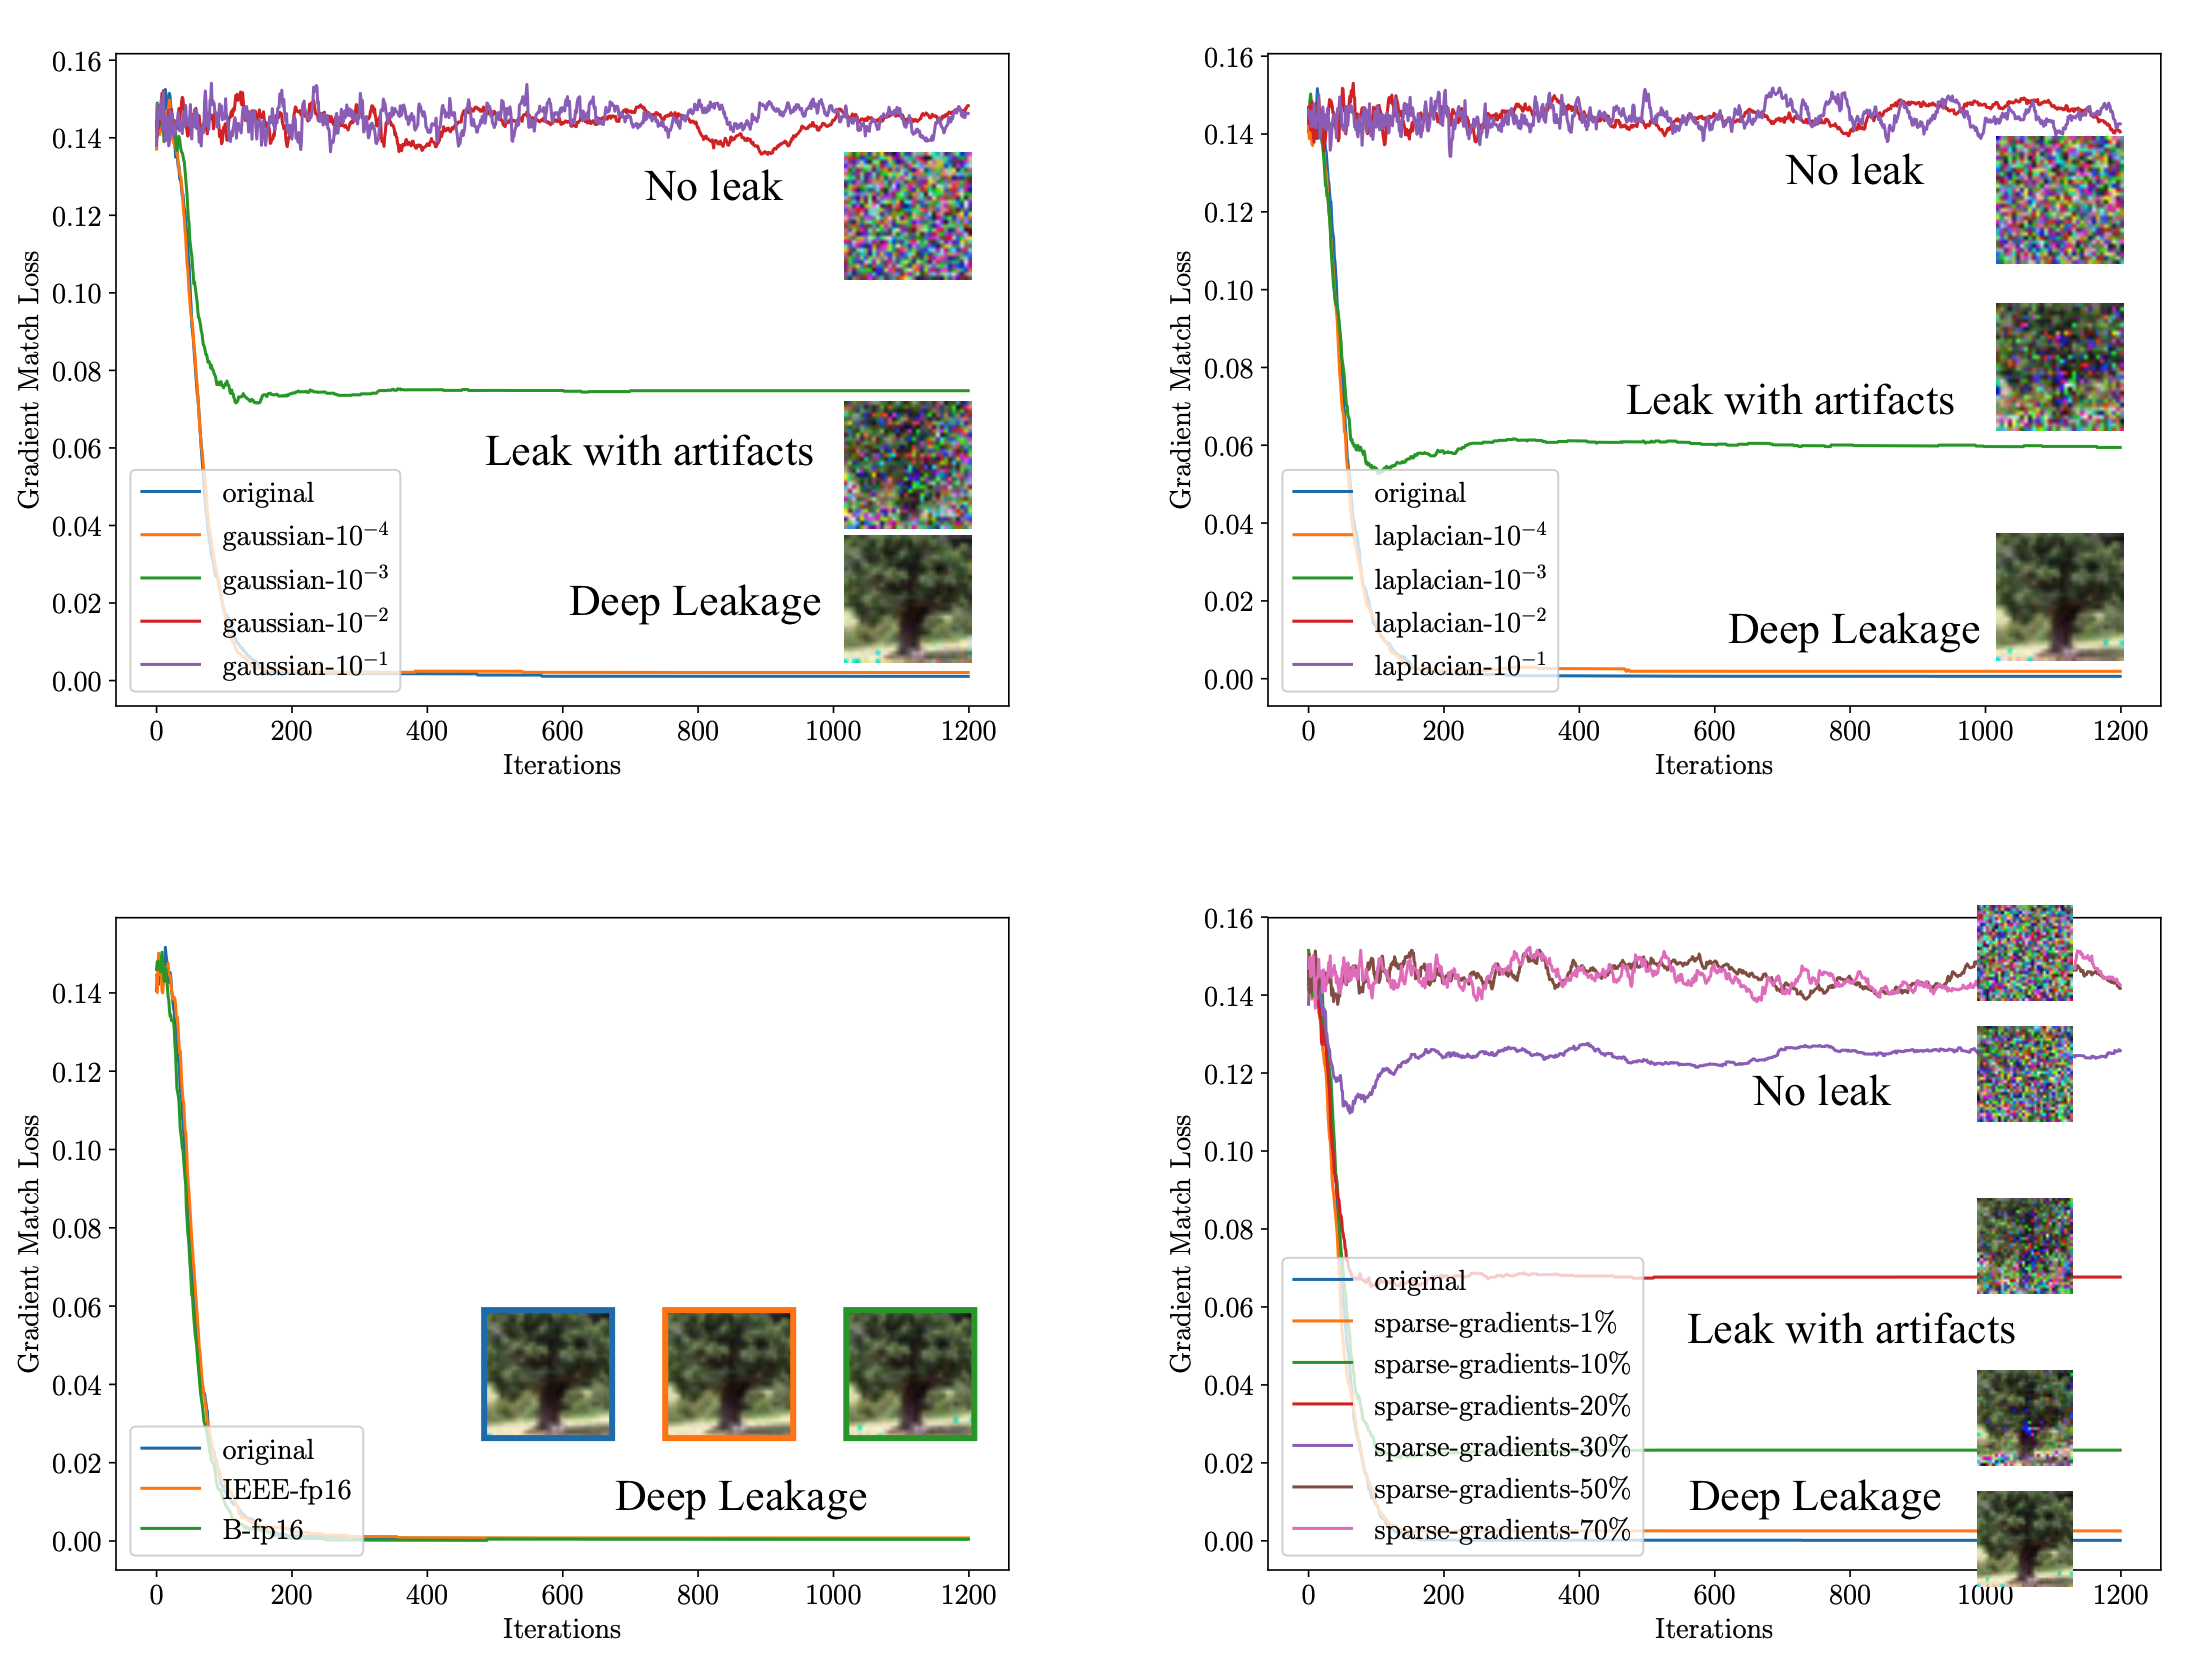
\includegraphics[width=\linewidth]{figures/fig4}
    % \caption{Caption \SH{font size should be as large as main text; reduce the space between the two rows}}
    \centering
    \begin{subfigure}[b]{0.49\textwidth}
        \centering
        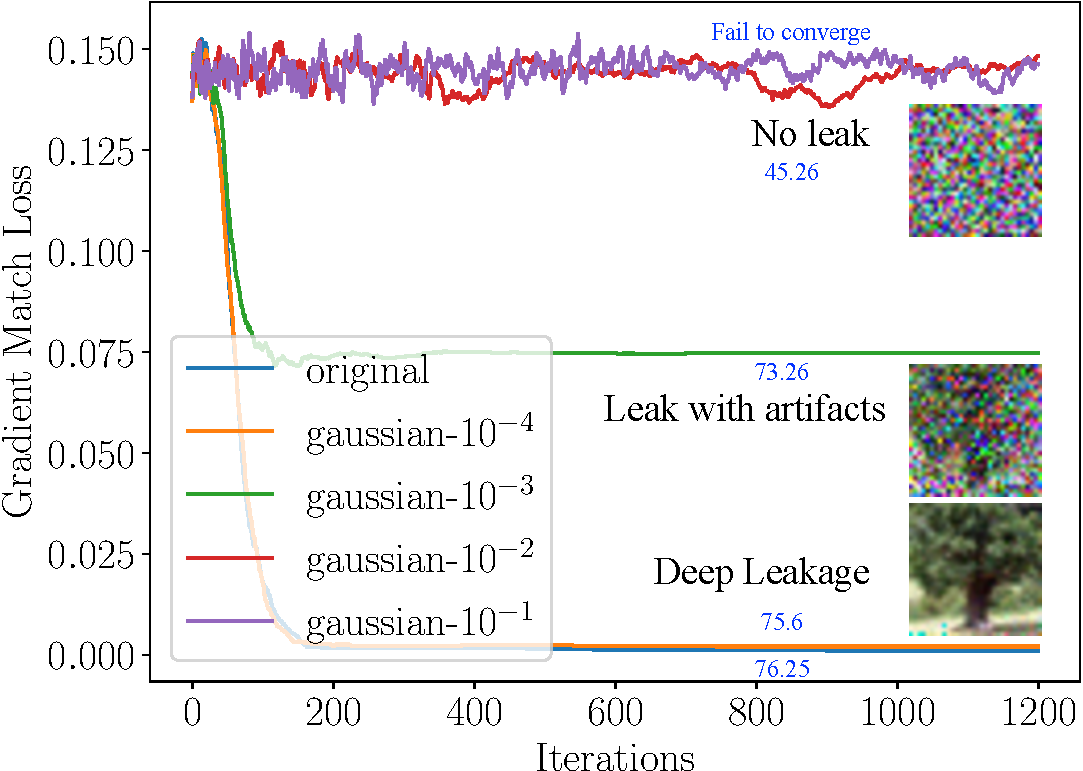
\includegraphics[width=\textwidth]{figures/fig5_gaussian-crop.pdf}
        \caption{Defend with different magnitude Gaussian noise.}
        \label{fig:defense:gaussian}
    \end{subfigure}
    \begin{subfigure}[b]{0.49\textwidth}
        \centering
        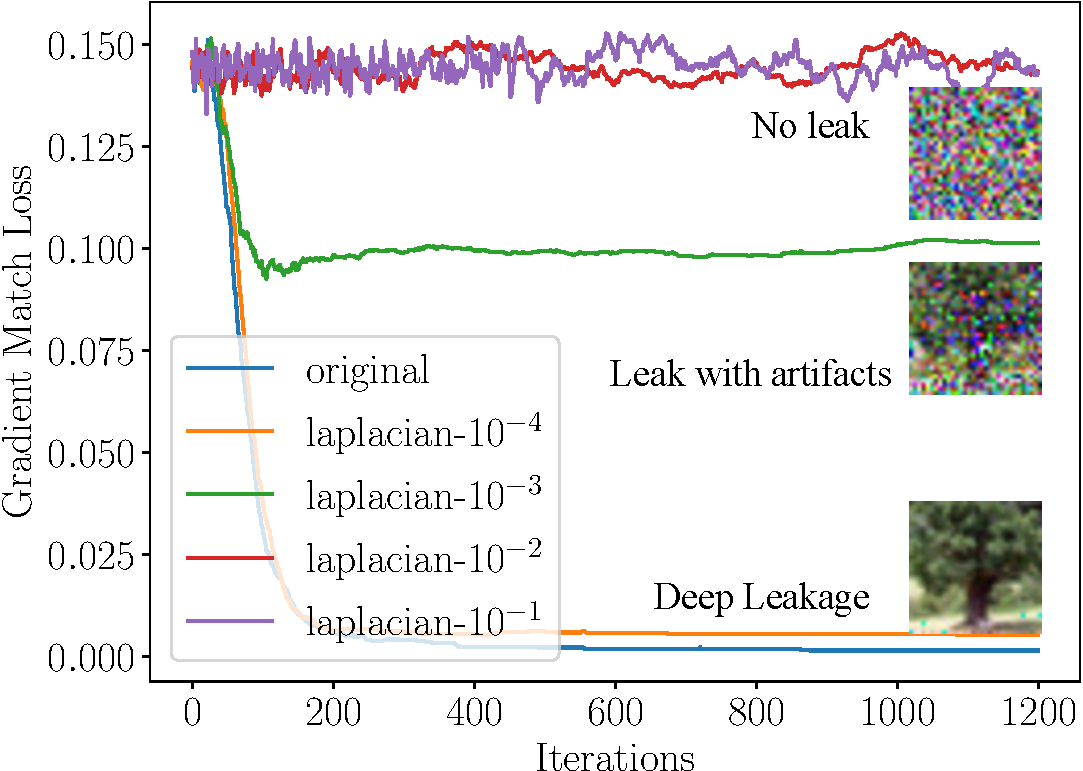
\includegraphics[width=\textwidth]{figures/fig5_laplacian-crop.pdf}
        \caption{Defend with different magnitude Laplacian noise.}
        \label{fig:defense:Laplacian}
    \end{subfigure} 
    \\ \vspace{4pt}
    \begin{subfigure}[b]{0.49\textwidth}
        \centering
        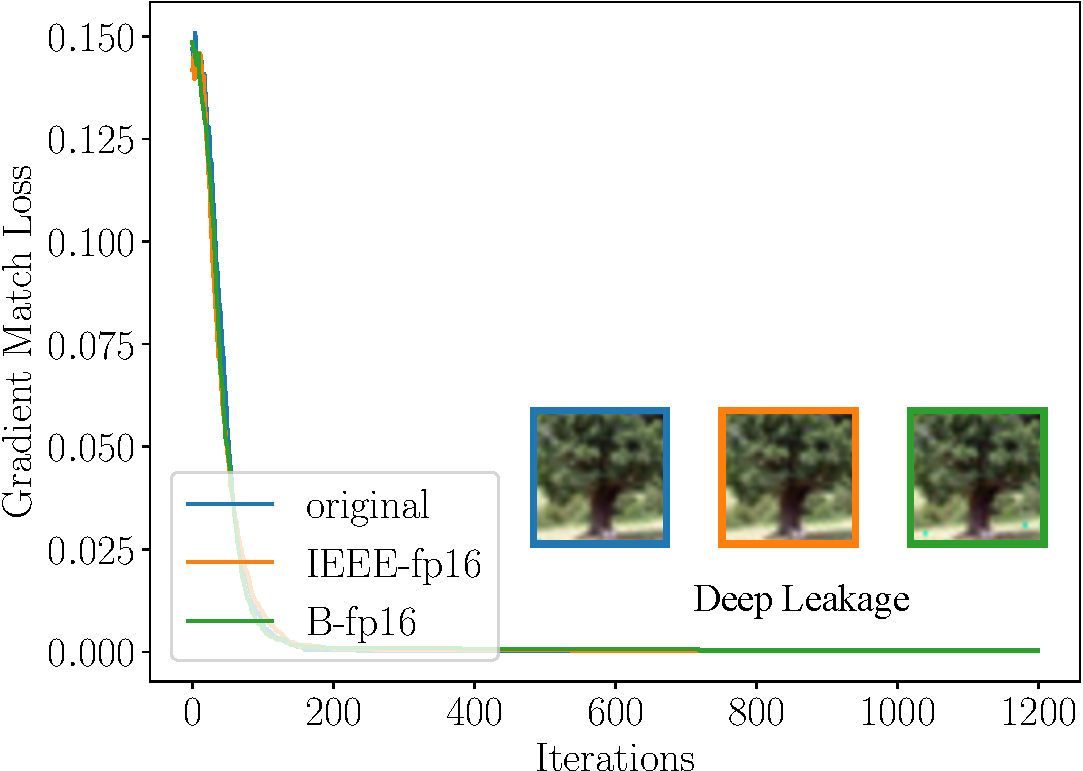
\includegraphics[width=\textwidth]{figures/fig5_fp16-crop.pdf}
        \caption{Defend with fp16 convertion.}
        \label{fig:defense:fp16}
    \end{subfigure}
    \begin{subfigure}[b]{0.49\textwidth}
        \centering
        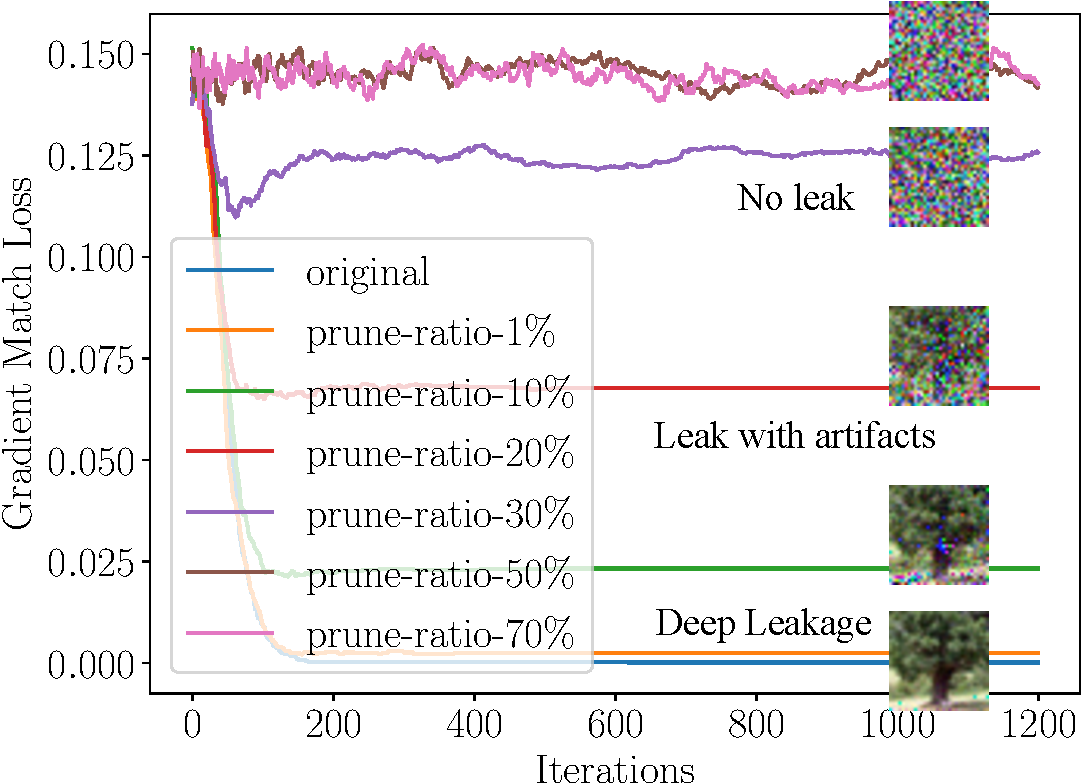
\includegraphics[width=\textwidth]{figures/fig5_dgc-crop.pdf}
        \caption{Defend with gradient pruning.}
        \label{fig:defense:dgc}
    \end{subfigure} 
    \caption{The effectiveness of various defense strategies. }
    \label{fig:defense}
    \vspace{-5pt}
\end{figure}
% 
\begin{table}[t]
\setlength{\tabcolsep}{3.5pt}
\centering
\footnotesize{
\begin{tabular}[t]{c||c||c|c|c|c||c|c|c|c||c}
    & Original  & \textbf{G}-$10^{-4}$ & \textbf{G}-$10^{-3}$ & \textbf{G}-$10^{-2}$ & \textbf{G}-$10^{-1}$  & \textbf{FP}-16  \\ \hline
    Accuracy & 76.3\% & 75.6\% & 73.3\% & 45.3\% & $\le$1\% & 76.1\% \\ \hline
    Defendability & -- & \lgxmark &  \lgxmark & \lgcmark &  \lgcmark & \lgxmark \\ \hline
    % 
    &     & \textbf{L}-$10^{-4}$ & \textbf{L}-$10^{-3}$ & \textbf{L}-$10^{-2}$ & \textbf{L}-$10^{-1}$  & \textbf{Int}-8  \\ \hline
    Accuracy & -- & 75.6\% & 73.4\% & 46.2\% & $\le$1\% & 53.7\% \\ \hline
    Defendability & -- & \lgxmark &  \lgxmark & \lgcmark &  \lgcmark & \lgcmark \\
\end{tabular}
}
\caption{The trade-off between accuracy and defendability. \textbf{G}: Gaussian noise, \textbf{L}: Laplacian noise, \textbf{FP}: Floating number, \textbf{Int}: Integer quantization.
\lgcmark~means it successfully defends against DLG while \lgxmark~means fails to defend (whether the results are visually recognizable). The accuracy is evaluated on CIFAR-100.
}
\label{tab:defense_vs_accuracy}
\vspace{-10pt}
\end{table}